\chapter{Evaluation der Arbeit}

In diesem Kapitel wird untersucht, ob die in Kapitel \ref{cha:Problemstellung} formulierte Forschungsfrage beantwortet wurde. Die zentrale Fragestellung lautete:

\textbf{"Wie kann eine Augmented-Reality-Anwendung f"ur mobile Smart-Geräte entwickelt werden, die Monteuren hilft, die korrekten Installationspositionen für Rauchmelder zu visualisieren und so die Einhaltung der Montagevorschriften sowie die Qualität und Effizienz des Installationsprozesses zu verbessern?"}

Zur Beurteilung der entwickelten Lösung werden die definierten Anforderungen und Bewertungskriterien herangezogen, die in Kapitel \ref{sec:requirements} festgelegt wurden.

\section{Visualisierung des Montageprozesses in einer AR-Umgebung}

Der entwickelte Prototyp implementiert die Visualisierung von virtuellen Objekten in einer Augmented-Reality-Umgebung für mobile Smart-Geräte. Zwar werden die Montageregeln nicht direkt an der Decke dargestellt, jedoch wird der Monteur durch den Prozess der Platzierung und Ausrichtung des Rauchmelders visuell unterstützt. Dadurch wird indirekt auf die korrekten Installationspositionen hingewiesen. Die Visualisierung erfolgt in Echtzeit und passt sich dynamisch an die Umgebung an. Der Monteur kann die Platzierung des virtuellen Rauchmelders nutzen, um vor der eigentlichen Montage zu prüfen, ob die gewählte Position den Vorschriften entspricht.

Potenzial zur Verbesserung besteht zum einen in der Qualität des virtuellen Rauchmelders. Hier könnte ein realistischeres 3D-Modell verwendet werden, um die Visualisierung noch authentischer zu gestalten. Zum anderen könnte der Ringindikator, der den Mindestabstand zu umgebenden Wänden anzeigt, verbessert werden. Aktuell wird der Indikator vollständig Rot beziehungsweise Grün gefärbt, je nachdem ob der Mindestabstand eingehalten wird oder nicht. Eine partielle Färbung könnte sofort erkennen lassen, an welchen Stellen der Mindestabstand nicht eingehalten wird.

Der Prototyp wurde ausschließlich im Portrait-Modus entwickelt, um die Interaktion mit dem Tablet zu erleichtern. Eine Implementierung im Landscape-Modus könnte jedoch die Visualisierung der Montageregeln verbessern, da das breitere Seitenverhältnis eine erweiterte Sicht auf die Umgebung ermöglicht. Besonders bei Smartphones führt der Landscape-Modus dazu, dass mehr von der Decke und anderen horizontalen Flächen im Sichtfeld liegt, was für bestimmte Anwendungsfälle vorteilhaft wäre.

\section{Praxistauglichkeit und Nutzererfahrung}

Die Anwendung wurde in einem realen Umfeld getestet und evaluiert. Dabei wurden verschiedene Szenarien simuliert, um die Funktionalität und Benutzerfreundlichkeit der Anwendung zu überprüfen. Die Anwendung konnte erfolgreich in verschiedenen Umgebungen eingesetzt werden und zeigte eine hohe Stabilität und Genauigkeit bei der Visualisierung der Montageregeln. Auch bei schwierigen Lichtverhältnissen oder unebenen Oberflächen funktionierte die Anwendung in den meisten Fällen.

Hier stellt vor allem die ,,Plug-and-Play''-Eigenschaft der Anwendung einen großen Vorteil dar. Der Benutzer kann die Anwendung starten und sofort mit der Interaktion beginnen, ohne dass eine manuelle Kalibrierung oder Initialisierung erforderlich ist. Dies trägt dazu bei, dass die Anwendung eine geringe Einstiegshürde aufweist und schnell einsatzbereit ist.

Fraglich ist jedoch, ob die Anwendung auch in größeren Räumen oder bei komplexeren Montagesituationen  eingesetzt werden kann. In solchen Fällen könnte die Tiefenmessung und das Tracking der Umgebung an ihre Grenzen stoßen. Auch die Platzierung von mehreren Rauchmeldern in einem Raum könnte die Leistung der Anwendung beeinträchtigen. Eine umfassende Evaluation in verschiedenen Umgebungen und Szenarien ist daher empfehlenswert, um die Leistungsfähigkeit der Anwendung zu überprüfen.

Zusätzlich besteht die Frage, ob die Anwendung bei erfahrenen Monteuren eher als Hilfsmittel oder als Störfaktor wahrgenommen wird. Es ist denkbar, dass erfahrene Monteure die Visualisierung der Montageregeln als überflüssig empfinden und sich dadurch in ihrer Arbeit eingeschränkt fühlen. 

Im Test wurden die Probanden mit folgender Aufgabe konfrontiert:
\begin{enumerate}
    \item Finde eine potenziell gültige Installationsposition für den Rauchmelder.
    \item Überprüfe, ob die Installationsposition den Montageregeln entspricht.
    \item Dokumentiere die Installationsposition mithilfe eines Bildes.
\end{enumerate}

Die Aufgabe wurde in verschiedenen Räumen durchgeführt. Im Durchschnitt benötigten die Probanden etwa 1,5 Minuten, um sie zu erfüllen. Mit der Anwendung konnte die korrekte Installationsposition jedoch bereits im ersten Durchgang in weniger als einer Minute gefunden werden. Im zweiten Durchgang ließ sich die Aufgabe sogar innerhalb weniger Sekunden lösen. Dies entspricht einer Zeitersparnis von rund 90\%. Ob sich dieser Effekt auch bei erfahrenen Monteuren zeigt, müsste durch weitere Tests überprüft werden.

\section{Umsetzung der Montageregeln}

Wie in Kapitel \ref{sec:ImplMontageregeln} beschrieben, wurde für den Prototypen eine Mindestanforderung an implementierten Montageregeln definiert. Es ist abzuwägen, welche der nicht integrierten Vorschriften für die Anwendung relevant sind und in zukünftigen Versionen berücksichtigt werden sollten. Hervorzuheben sind dabei die Montage an schrägen Decken und der Mindestabstand zu Decken-, Boden- und Wandöffnungen für Kühl- und Heizungsaus- und -einlässe. Diese Regeln sind besonders wichtig, da sie die Funktionalität der Rauchmelder beeinträchtigen können, wenn sie nicht eingehalten werden. Die Implementierung dieser Montageregeln könnte die Anwendung noch nützlicher machen und dem Benutzer eine umfassendere Unterstützung bei der Installation von Rauchmeldern bieten.

Insgesamt ist festzuhalten, dass die Umsetzung der Montageregeln in der Augmented-Reality-Umgebung erfolgreich war. Das Framework, das für die Implementierung der Montageregeln entwickelt wurde, stellt eine solide Grundlage für zukünftige Erweiterungen dar und ermöglicht eine einfache Integration weiterer Regeln und Richtlinien.

\section{Bewertung der Performance}

Die Performance der Anwendung wird anhand verschiedener Kriterien bewertet, darunter Bildrate, Latenz und Stabilität. Getestet wurde die Anwendung auf einem iPad Pro (11 Zoll, 3. Generation) mit M1-Chip.

Die durchschnittliche Bildrate beträgt 59 FPS (Frames per Second), was für eine flüssige Darstellung der AR-Szene vollkommen ausreicht. Wie bereits erwähnt, kann es bei der Platzierung des virtuellen Rauchmelders zu kurzen Verzögerungen kommen. Diese sind jedoch minimal und beeinträchtigen die Benutzererfahrung nicht. Gelegentlich treten Drift-Effekte auf, die in der Regel schnell von ARKit korrigiert werden.

Während der Tests kam es nur selten zu Abstürzen oder schwerwiegenden Fehlern. Die Stabilität der Anwendung ist insgesamt als gut zu bewerten. In Einzelfällen traten Fehler auf, die einen Neustart der AR-Anwendung erforderlich machten. In den meisten Fällen konnte die Anwendung jedoch problemlos weiterverwendet werden.

\section{Bekannte Schwachstellen und Verbesserungspotenzial}

Trotz der positiven Ergebnisse gibt es noch einige Schwachstellen und Verbesserungspotenziale, die in zukünftigen Versionen der Anwendung berücksichtigt werden sollten.

Die Genauigkeit der Tiefenmessung ist ein entscheidender Faktor für die Umsetzung der Montageregeln. Der Prototyp konnte eine Genauigkeit von etwa 1-2 cm erreichen (siehe Abbildung \ref{fig:DistanceIndicator}). Dies wurde als ausreichend angesehen, um die Montageregeln präzise zu visualisieren. 

\begin{figure}[ht]
    \centering
    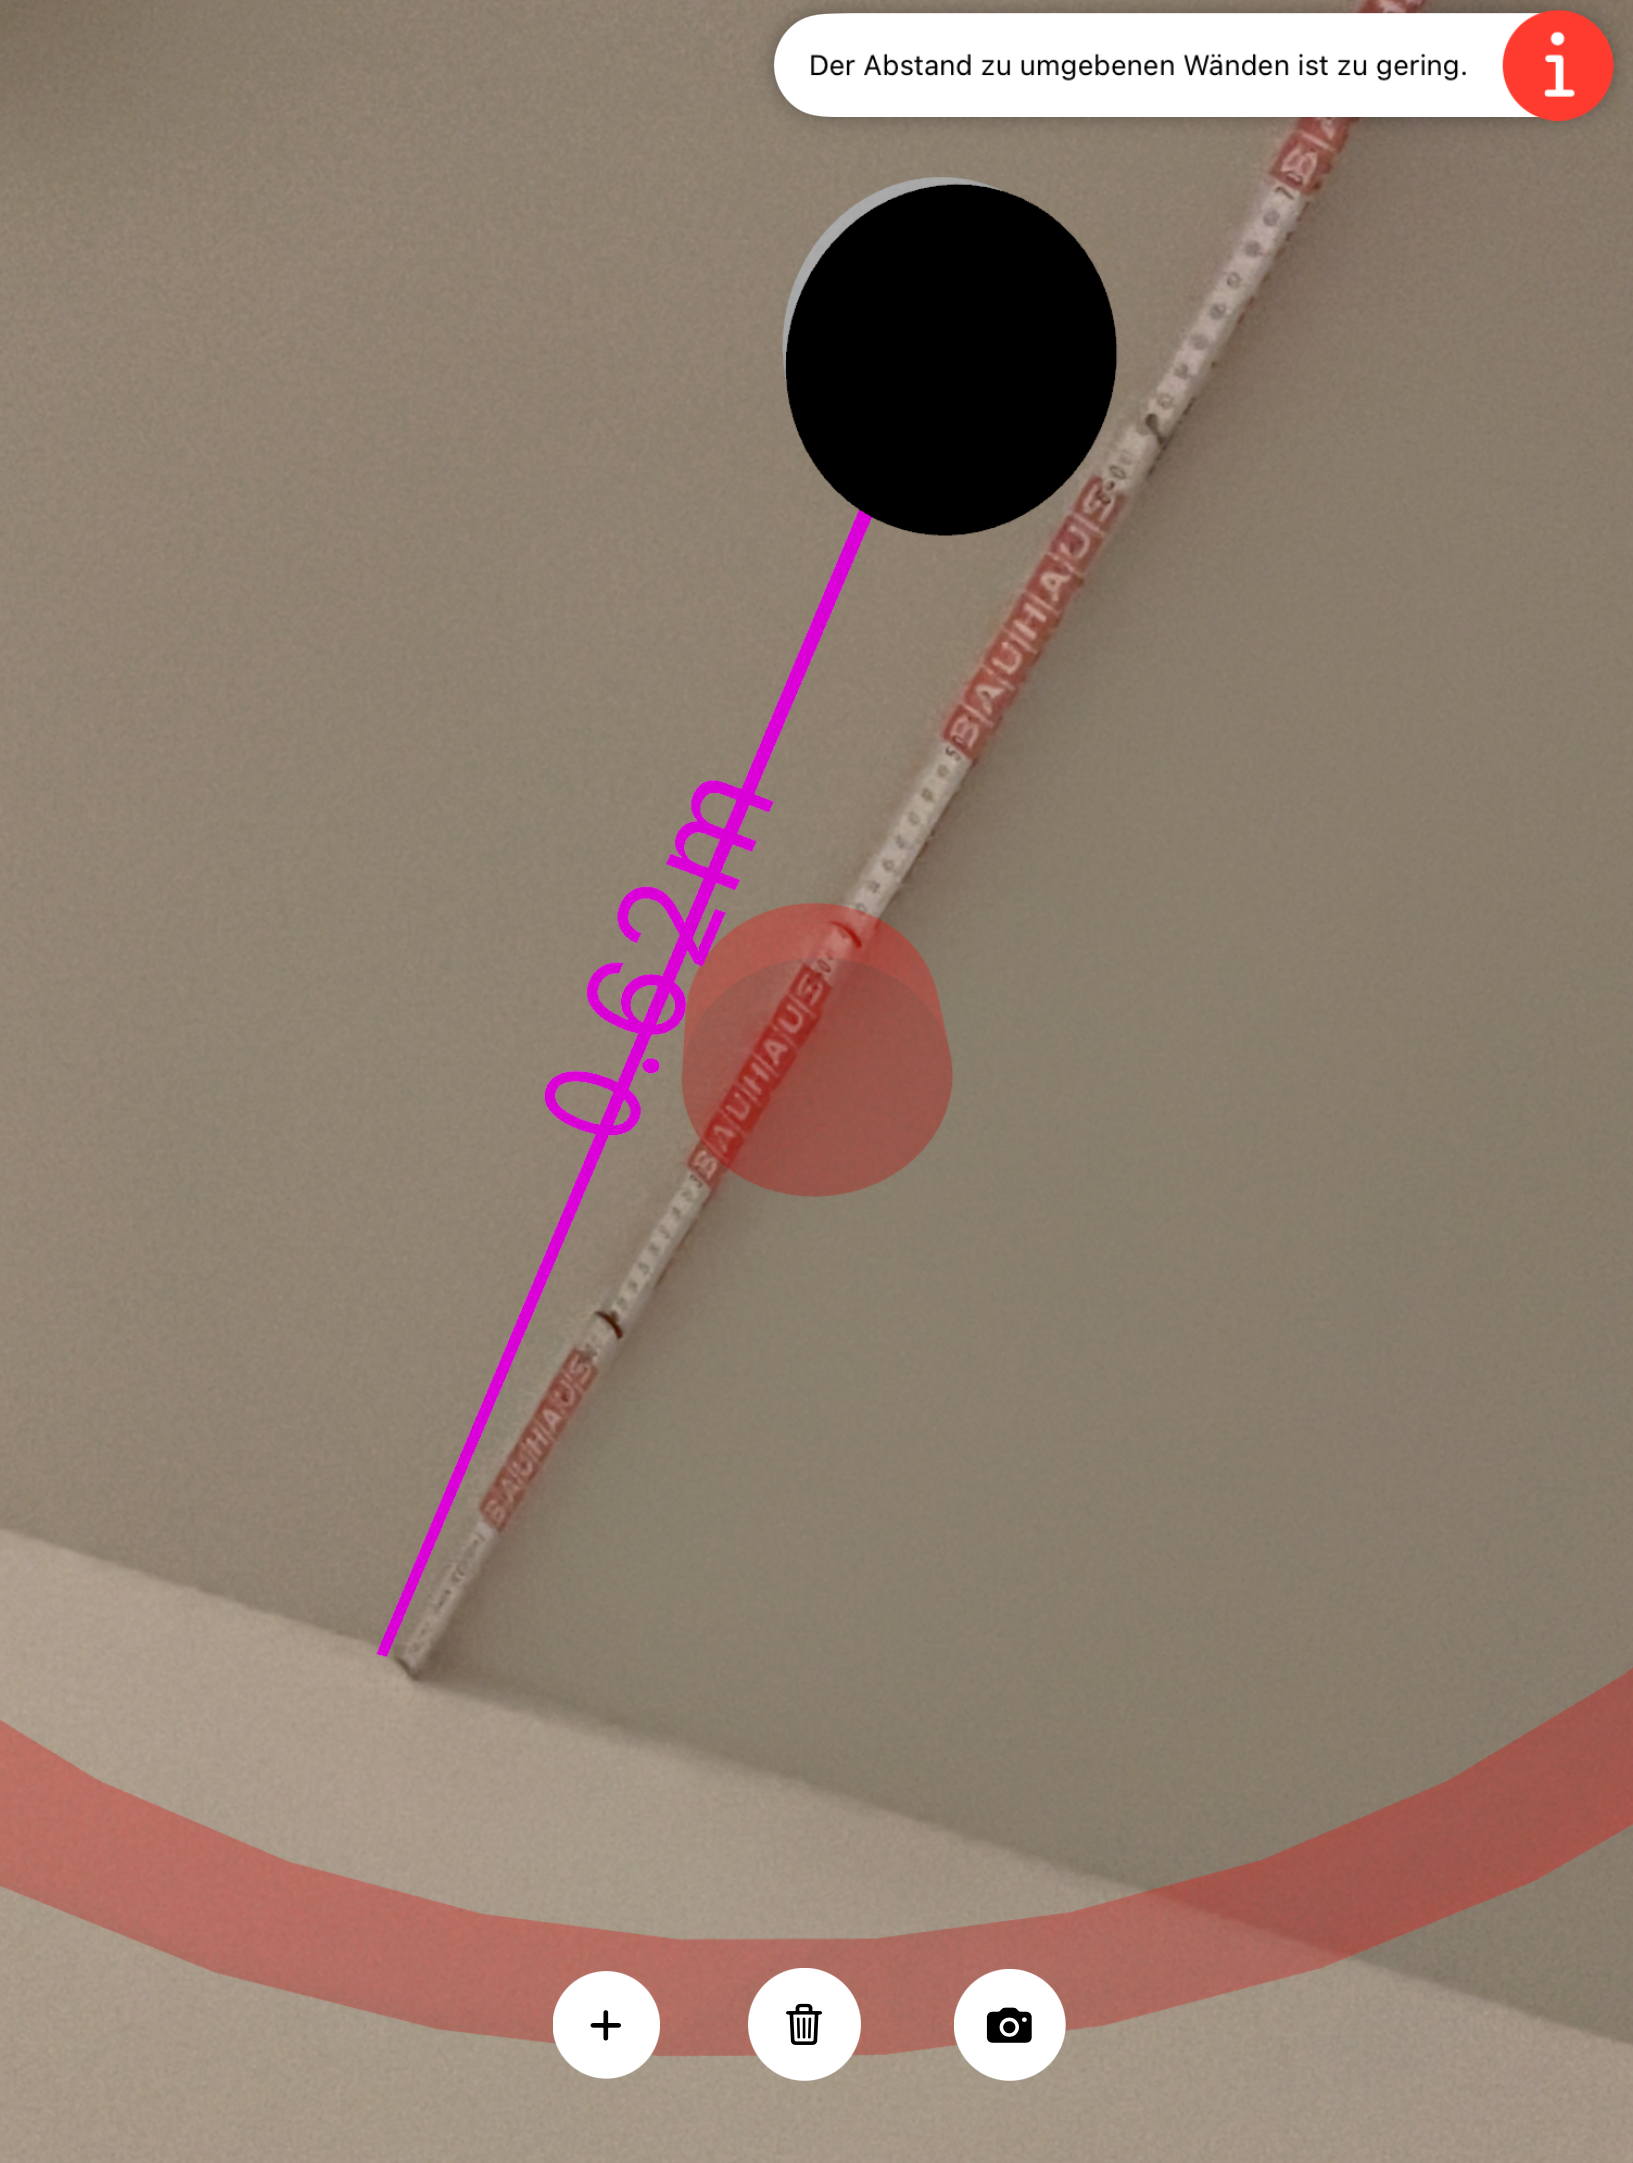
\includegraphics[width=0.5\textwidth]{DistanzIndikator}
    \caption{Genauigkeit der Tiefenmessung}
    \label{fig:DistanceIndicator}
\end{figure}

Fraglich ist, ob diese Genauigkeit auch in komplexeren Umgebungen oder bei größeren Räumen gewährleistet werden kann, da die LiDAR-Sensoren der Apple-Geräte eine begrenzte Reichweite der Tiefenmessung aufweisen. Die Reichweite der Sensoren beträgt etwa 5 Meter. Eine umfassende Evaluation der Genauigkeit in verschiedenen Szenarien ist daher empfehlenswert. Zudem besteht die Frage, ob die von der Anwendung generierten Screenshots als eindeutiger Nachweis einer korrekten Installation genutzt werden können. \cite{appledevdoc}